\section{Misure di temperatura mediante termocoppia}
\paragraph{Dati e richieste}
Vengono fornite due serie di misure di temperatura allo scarico di una camera di combustione, eseguite mediante termocoppia di tipo B. La prima è costituita da 1599 valori ("Serie corta"), la seconda da 9999 ("Serie lunga"). Entrambe le serie sono campionate con una frequenza di campionamento di 100 Hz e vengono fornite mediante file testuale (.txt).\\
Si chiede di svolgere l'analisi statistica dei dati.
\subsection{Risoluzione}
Si riportano i risultati emersi dall'elaborazione dei dati sperimentali. I calcoli sono stati svolti mediante il software \textit{Matlab} e le funzioni built-in.
\paragraph{Suddivisione in classi e istogramma}
Entrambe le serie sono divise in 10 classi, di uguale ampiezza, costruite affinché non ci possa essere ambiguità nell'attribuzione dei valori: poiché le misure hanno 6 cifre decimali, gli estremi di classe sono definiti con 7 cifre decimali. L'estremo della prima classe viene scelto come il minimo valore di \gls{symb:T} a cui viene sottratto 0.5e-7 \textsuperscript{o}C. Analogamente, l'estremo superiore dell'ultima classe viene calcolato sommando la stessa quantità al massimo valore di \gls{symb:T} nella serie. I valori estremi delle due serie sono mostrati in Tab.\ref{tab:estremitemp}, riportati integralmente per mettere in evidenza il numero di cifre decimali.
\begin{table} [H]
	\centering
	\begin{tabular}{c|c|c}
		\toprule
		\toprule
		\textbf{Serie} & \textbf{\textit{T\textsubscript{MIN}} [\textsuperscript{o}C]} &\textbf{\textit{T\textsubscript{MAX}} [\textsuperscript{o}C]} \\
		\midrule
		\midrule
		Corta & 953.745910 & 1193.110960\\
		\midrule
		Lunga & 931.352290 & 1449.917970 \\
		\bottomrule
		\bottomrule
	\end{tabular}
\caption{Valori estremi di temperatura}
\label{tab:estremitemp}
\end{table}
Gli istogrammi relativi alle due serie sono mostrati in Fig.\ref{fig:istboth}.
\begin{figure} [H]
	
	\begin{subfigure}{0.49\textwidth}
		\centering
		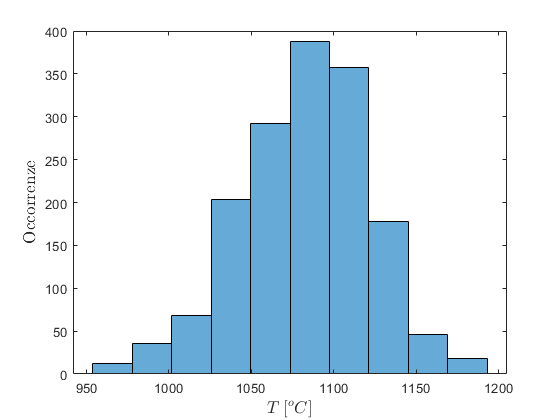
\includegraphics[width=0.99\linewidth]{chapters/1-misureT/istogrammashort}
		\caption{Serie corta}
		\label{fig:istogrammashort}
	\end{subfigure}%
	\begin{subfigure}{0.49\textwidth}
		\centering
		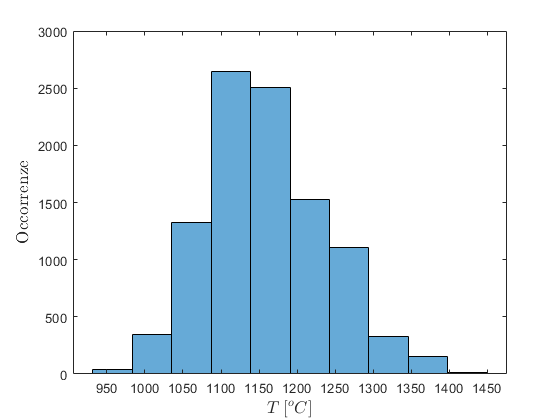
\includegraphics[width=0.99\linewidth]{chapters/1-misureT/istogrammalong}
		\caption{Serie lunga}
		\label{fig:istogrammalong}
	\end{subfigure}
\caption{Istogrammi delle due serie}	
\label{fig:istboth}
\end{figure}
Si osserva come entrambe le distribuzioni di dati siano simili alla distribuzione gaussiana, mostrando tuttavia una evidente asimmetria. Quest'ultima è quantificabile dal coefficiente di skewness, riportato in Tab.%\ref{}.
\paragraph{Calcolo delle frequenze relative e cumulate}
Successivamente vengono riportate delle rappresentazioni grafiche 
delle frequenze relative (\gls{symb:f}) e frequenze cumulate normalizzate(\gls{symb:F}) delle varie classi.



\begin{figure}
	
	\begin{subfigure}{0.5\textwidth}
		\centering
		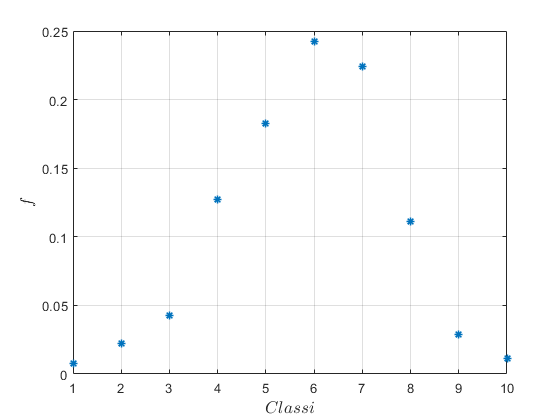
\includegraphics[width=\linewidth]{chapters/1-misureT/relshort}
		\caption{Serie corta}
		\label{fig:relshort}
	\end{subfigure}%
	\begin{subfigure}{0.5\textwidth}
		\centering
		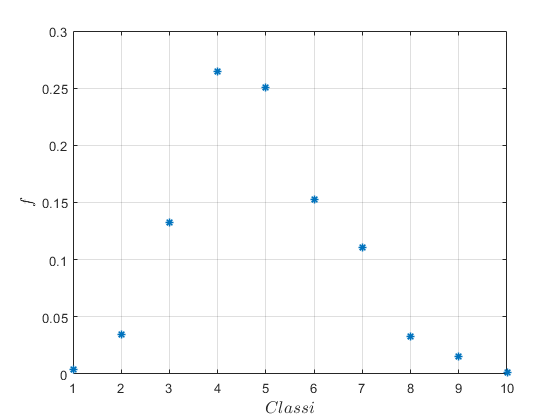
\includegraphics[width=\linewidth]{chapters/1-misureT/rellong}
		\caption{Serie lunga}
		\label{fig:rellong}
	\end{subfigure}
	\caption{Frequenze relative delle diverse classi}
	\label{fig:relboth}
\end{figure}

\begin{figure}
	\centering
	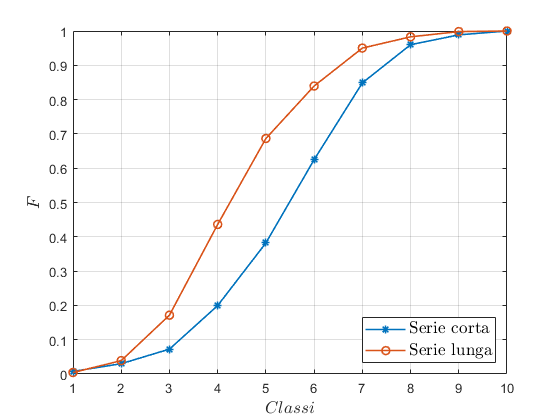
\includegraphics[width=0.7\linewidth]{chapters/1-misureT/cumboth}
	\caption{Frequenze cumulate normalizzate per entrambe le serie}
	\label{fig:cumboth}
\end{figure}


\paragraph{Calcolo degli indici statistici}
L'analisi statistica dei dati viene svolta mediante il calcolo degli indici statistici relativi alle due serie di dati. In particolare, si riportano media (\gls{symb:Tmean}) e mediana (\gls{symb:Tmed}) delle due serie, nonché deviazione standard (\gls{symb:sigmaT}) e skewness (\gls{symb:skew}) delle distribuzioni. I risultati sono presentati in Tab.\ref{tab:indicistat}.

\begin{table} [H]
	\centering
	\begin{tabular}{c|c|c}
		\toprule
		\toprule
		\textbf{Indice} & \textbf{Serie corta}&\textbf{Serie lunga}\\
		\midrule
		\midrule
		$\overline{T}$ [\textsuperscript{o}C]& 1082.8 & 1159.2\\
		\midrule
		$T_\textit{MEDIANA}$ [\textsuperscript{o}C]&1085.7&1152.4\\
		\midrule
		$\sigma_T$ [\textsuperscript{o}C]&39.147 & 77.841\\
		\midrule
		$SK$ & -0.27 & 0.40 \\
		\bottomrule
		\bottomrule
	\end{tabular}
\caption{Indici statistici delle due distribuzioni}
\label{tab:indicistat}
\end{table}

\paragraph{Stima dell'errore statistico}
Lo studio statistico delle due serie di dati si conclude con la stima dell'errore statistico (\gls{symb:Estat}).  Risulta necessario calcolare la deviazione standard del valore medio di temperatura (\gls{symb:sigmaTmean}) secondo:
\begin{equation}
	\sigma_{\overline{T}} = \frac{\sigma_{T}}{\sqrt{N}} \label{eq:sigmaTmean}
\end{equation}
dove \gls{symb:N} è il numero di campioni di ciascuna serie.
Infine, il valore di \gls{symb:Estat} si ottiene con:
\begin{equation}
	\epsilon_{\textit{STAT}}=\sigma_{\overline{T}}\,t_{\textit{95\%}}
\end{equation}
dove \gls{symb:t95} è ricavato dalla distribuzione t per un intervallo di confidenza al 95\% (dove \gls{symb:nu} = \gls{symb:N} - 1, dove 1 rappresenta il numero di gradi di libertà persi a seguito dell'introduzione di \gls{symb:Tmean}).
\begin{table} [H]
	\centering
	\begin{tabular}{c|c|c}
		\toprule
		\toprule
		\textbf{Indice} & \textbf{Serie corta}&\textbf{Serie lunga}\\
		\midrule
		\midrule
		$t_{\textit{95\%}}$ &1.9614&1.9602\\
		\midrule
		$\nu$ & 1598 & 9998\\
		\midrule
		$\epsilon_{\textit{STAT}}$  [\textsuperscript{o}C]& $\pm $1.9202 &  $ \pm$ 1.5259\\
		\bottomrule
		\bottomrule
	\end{tabular}
	\caption{Errore statistico delle due distribuzioni}
	\label{tab:errorestat}
\end{table}

Da Tab.\ref{tab:errorestat} si nota come un numero elevato di campioni garantisca un errore statistico molto contenuto, che risulta minore di \gls{symb:sigmaT} di un ordine di grandezza. Questo risultato deriva dalla presenza di $\sqrt{N}$ in Eq.(\ref{eq:sigmaTmean}), il cui valore ammonta a $\sim$ 40 per la prima serie, a $\sim$ 100 per la seconda. Per quanto riguarda il valore di \gls{symb:t95}, si osserva che tende al valore asintotico ($\nu \rightarrow \infty $) di 1.960 in entrambi i casi, quindi l'influenza di tale parametro sull'errore statistico è pari per le due serie.